\documentclass[a4paper]{IEEEtran}

\usepackage[utf8]{inputenc} % UTF-8
\usepackage[T1]{fontenc} % 8-bit fonts

\usepackage{lmodern} % Modern font

\usepackage{xcolor} % Colors
\usepackage{hyperref} % URLs
\usepackage{graphicx} % Graphics

\usepackage{booktabs} % Formal tables
\usepackage{multirow} % Table cells that span multiple rows
\usepackage{colortbl} % Table cell coloring

%\usepackage{pgfplots} % Graph plots
%\usepackage{pgfplotstable} % Table plots

\newcommand\TODO{\textcolor{red}{[TODO]}}
\newcommand\todo[1]{\textcolor{red}{[TODO: #1]}}
\newcommand\CN{\textcolor{blue}{[Citation Needed]}}
\newcommand\cn[1]{\textcolor{blue}{[Citation Needed: #1]}}

\title{The Cellular Automata Research Platform: \\ Communication and Verification}
\author{Per Thomas Lundal, \emph{Norwegian University of Science and Technology}}
\markboth{TDT4501 - Computer Science Specialization Project, Autumn 2014, Supervised by Gunnar Tufte}{}

\begin{document}

\maketitle

\begin{abstract}

    %Evolvable hardware is... \TODO
%
Research into evolvable hardware has long been performed at NTNU.
In 2003, a cellular automata research platform was created with the use of an FPGA.
It was based on a two-dimensional matrix of sblocks, with built-in support for development.

In expectation of new hardware with a larger FPGA, the platform was updated and extended in 2014.
It was optimized to provide a speedup of 4 for most operations by taking advantage of increased resources.
%The addition of a DFT and extension of the sblock matric into three dimensions were also promising new features.
However, since the hardware did not arrive in time, the new PCI Express interface was not implemented.
This also meant that new design could only be verified in simulation.

The goal of this project was to finalize the platform, such that the new features and improved speed could be taken advantage of.
The first objective towards that end was to replace the old communication interface.
The second was to verify that the new design worked correctly when implemented in hardware.

%Since the desired hardware was still unavailable at the start of this project, similar hardware with a smaller FPGA was procured instead.
%Although the maximum size of the sblock matrix was greatly reduced, it would allow for implementation of the new communication interface and verification of the design.

This paper details the implementation of the new communication interface, both in hardware and software.
Then, the previously upgraded design is implemented and tested in the new hardware.

Implementation of the new communication interface is a success.
However, testing shows that there are a lot of issues with the upgraded design.
Some issues were possible to fix within the alotted time, but several critical remain.

%\todo{shorten this some?}



\end{abstract}

\section{Introduction}

    \TODO


\section{Background}

    \subsection{Evolvable hardware}

Evolvable hardware (EHW) is a field of science where evolutionary algorithms (EAs) are used in the creation of specialized hardware.
Taking inspiration from nature, artificial evolution is 

Evolvable hardware was born out of the desire to take advantage of principles of biological systems for computation.

\todo{rewrite}

Evolution:
Principles of life
Genetic Algorithms
Evolution in materio/silicon \cite{miller2014evolution}

Development:
\cite{harding2008artificial} \cite{tufte2008evodevo}
Zygote
Scalability
Robustness
Plasticity

\subsection{Cellular automata}

\todo{resembles biological stuff}

A cellular automaton (CA) is a structure made up of vast numbers of very simple computational units called cells.
The cells are arranged in a grid, with communication only permitted between nearby cells according to a neighborhood.
The von Neumann neighborhood is common for two-dimensional CAs \CN;
It includes the cells to the north, south, east and west, along with itself (center).
An example of this is shown in \figurename~\ref{fig:ca}.

\begin{figure}[!ht]
    \centering
    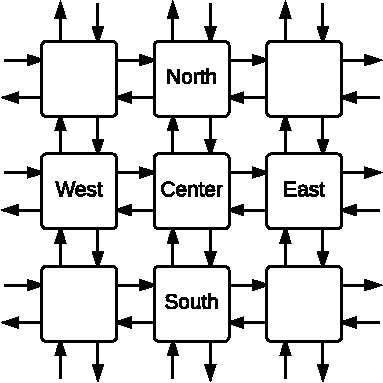
\includegraphics[width=0.25\textwidth]{figures/ca}
    \caption{An excerpt from a 2D CA using a von Neumann neighborhood. All outputs from a given cell carries the same value.}
    \label{fig:ca}
\end{figure}

Each cell has a state, which is often a binary number where 1 represents alive and 0 represents dead.
At each discrete time step, each cell updates its state based on the states in its neighborhood.
The update function is often specified as a look-up-table (LUT), where the next state is defined for all possible neighborhood states\footnotemark.
\footnotetext{
    The length of the LUT increases exponentially with the size of the neighborhood.
    $L=S^N$ where $L$ is the LUT length, $S$ is the number of possible states and $N$ is the number of cells in the neighborhood.
}
If all cells implement the same update function then the CA is uniform, otherwise it is non-uniform.

CAs have been shown to be Turing complete \cite{neumann1966selfreplication, codd1968cellular}, which means they are able to perform any kind of computation.


Usage in EHW:
Langton's research on emergent computation and phase transition \cite{langton1990edgeofchaos}.
Wolfram's four qualitative CA classes \cite{wolfram1984complexity}.

Due to their resemblance to biological systems, CAs have been 

Self-Replication:
von Neumann's work on self-replication from around 1950 \cite{neumann1966selfreplication}.
Self-replicating structures \cite{reggia1998neumann}.
Replicating universal computers with 63 states and 8500 rules \cite{perrier1996toward}.

\subsection{Field Programmable Gate Array}

A Field Programmable Gate Array (FPGA) is a type of reconfigurable hardware.
It can implement any desired logical operation by configuring and connecting a number of look-up tables (LUTs) and flip-flops (FFs).
FPGAs can also contain dedicated blocks for adding, multiplying, random access memory (RAM) and other functions.
Configurable elements are grouped into configurable logic blocks (CLBs), which through a network of interconnects can be connected to each other or input/output pins.
An example of this structure is shown in \figurename~\ref{fig:fpga}.
Note that modern FPGAs consists of thousands of CLBs and hundreds of I/O pins \cite{ds160}.

\begin{figure}[!ht]
    \centering
    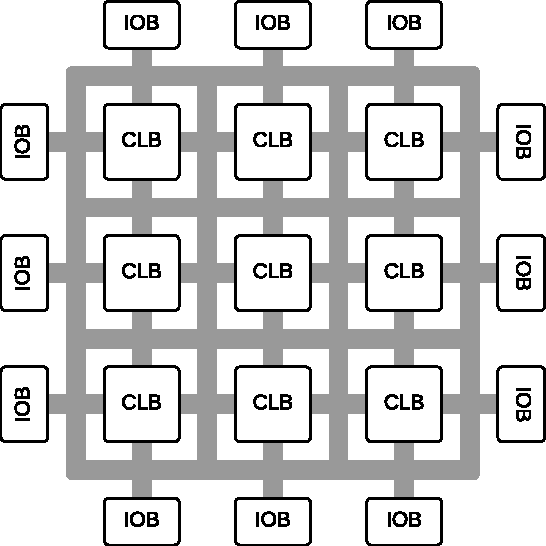
\includegraphics[width=0.30\textwidth]{figures/fpga}
    \caption{High-level block diagram of an FPGA. An array of configurable logic blocks (CLBs) and input/output blocks (IOBs) are connected by a network of interconnects.}
    \label{fig:fpga}
\end{figure}

FPGAs have been the subject of EHW research due to their reconfigurability, and several researchers have been successful in evolving working electronic circuits \cite{huelsbergen1998evolution, thompson1997evolved}.
However, the resulting circuits have often ended up using intrinsic properties of the silicon and been very sensitive to environmental changes.

The trouble with using modern FPGAs for EHW research is that some configuration bitstrings can destroy the FPGA \cite{ug380, xapp151}.
This means that the bitstring can not be used directly as the genotype without complicated tests to discard the dangerous bitstrings.
One solution to this problem is the sblock. \todo{does this sentence fit in here?}

\subsection{Sblock}

\begin{itemize}
    \item Haddow: \cite{haddow2000sblock}
    \item Basicly a configurable CA
    \item Virtual FPGA
    \item Add figure
\end{itemize}

\begin{figure}[!ht]
    \centering
    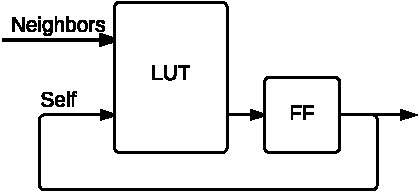
\includegraphics[width=0.25\textwidth]{figures/sblock}
    \caption{Detailed block diagram of an sblock. The LUT can be reconfigured on-the-fly to implement any logical function.}
    \label{fig:sblock}
\end{figure}

\subsection{PCI Express}

The PCI Express interface was designed to tackle the arising trouble with clocked parallel buses like PCI.
The problem with such buses is that the clock speed can not be increased beyond a given threshold, as the slightly different lengths of the many wires causes data to arrive at slightly different times.
Reducing the clock period to less than the variation in arrival time means the data will become corrupted.
This problem is exacerbated with increasing bus size.

PCI Express is therefore based on serial communication over differential pairs (lanes \footnote{
        PCI Express operates in full duplex mode, which means that each lane has an independent differential pair in each direction.
        1, 2, 4, 8, 16 or 32 lanes are supported, but data is striped and thus still transmitted serially.
    }) without the need for a reference clock \cite{pcie}.
This allows an extremely fast clock speed compared to a parallel bus, and much greater bandwidth in total.
PCI Express consists of three layers; the physical layer, the data link layer and the transaction layer, structured as shown in \figurename~\ref{fig:pcie}.

\begin{figure}[!ht]
    \centering
    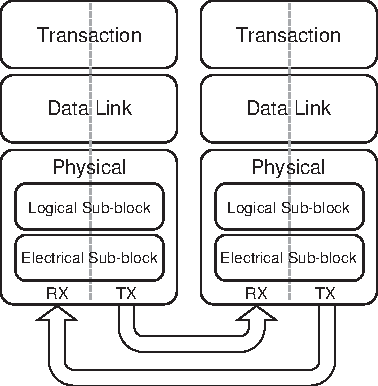
\includegraphics[width=0.25\textwidth]{figures/pcie}
    \caption{High-level diagram showing the layered structure of PCI Express. (Reprinted from \cite{pcie})}
    \label{fig:pcie}
\end{figure}

The transaction layers primary responsibility is the creation and parsing of transaction layer packets (TLPs).
TLPs are used to trigger events or start various transactions, most commonly to initiate read and write requests \footnote{
        Read and write requests are directed at one of up to six base address registers (BARs).
        They represent internal memory areas that can be anywhere from a few bytes to several gigabytes in size.
    }.
Most requests entail the return of a completion TLP containing the requested data or other information.
TLPs consists of multiple 32-bit double words (DW), where the first is a common header describing the type of packet.

The data link layer ensures integrity by adding error detection codes to outgoing TLPs and performing error detection and correction on incoming TLPs.
It is also responsible for retransmission if corruption occurs.

The physical layer is responsible for serialization and deserialization of the data stream.
Each byte is padded with two extra bits (8b/10b encoding) to allow clock recovery.



\section{Previous Work}

    The Cellular Automata Research Platform (CARP) has been the subject of three previous master theses at NTNU.
The original implementation was made by Djupdal in 2003.
It was then extended with a range of various output methods by Aamodt in 2005.
Finally, it was further extended and optimized in expectation of new hardware by Støvneng in 2014.

\subsection{Conception}

In 2002, NTNU invested in a CompactPCI computer with a NallaTech BenERA FPGA board to be used for research within the field of evolutionary hardware.
The task of developing a platform for the system, based on a matrix of sblocks, fell to Djupdal \cite{djupdal2003sblock}.

An overview of the resulting hardware platform is shown in \figurename~\ref{fig:overview-djupdal}.
It consists of the mentioned sblock matrix, block RAM (BRAM) for storing the state and type of each cell, a development unit, control logic, and a PCI communication unit.

\begin{figure}[!ht]
    \centering
    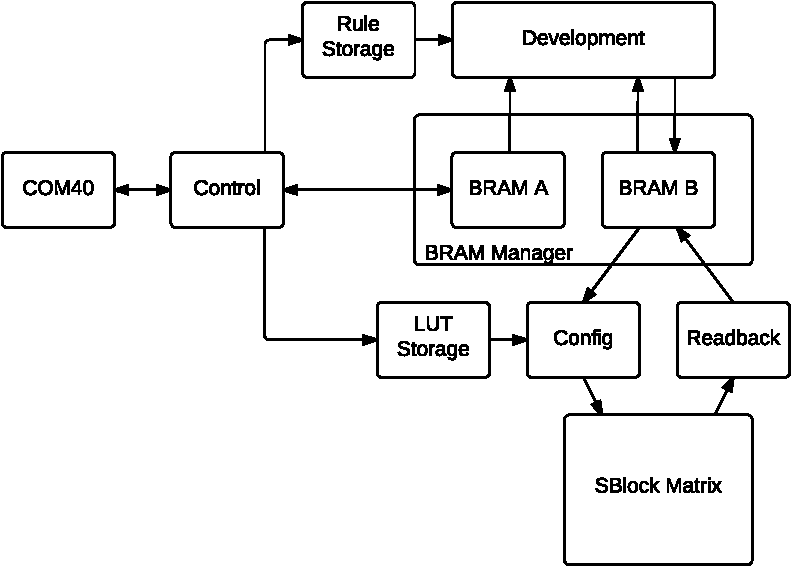
\includegraphics[width=0.48\textwidth]{figures/overview-djupdal}
    \caption{High-level block diagram of the hardware platform after Djupdal's original work.}
    \label{fig:overview-djupdal}
\end{figure}

The system is meant to be controlled by a computer running a genetic algoritm.
A common flow of operation is to initialize the system with the genotype, develop it into its phenotype, run the SBM, and send the new states back to the computer.
The computer then uses the newly received state data to calculate a fitness score.

The system is initialized by writing states and types to BRAM A, in addition to storing development rules and LUT conversion rules.
Then a development step can be performed by reading cell types from BRAM A\footnotemark, testing development rules, and writing the (possibly changed) types back to BRAM B.
\footnotetext{
    After the first 8 rules have been tested on all cells, center cell types are read from BRAM B instead.
    This is needed to prevent the result of a rule in an earlier iteration from being deleted if no rules trigger in a later iteration.
}
The development unit tests 8 rules on 2 cells each cycle in raster order.
Optionally, the BRAMs can be logically swapped and further development steps performed.
The SBM can then be configured by translating the types in BRAM B into LUT entries according to the LUT conversion rules, before being run for a desired amount of cycles.
Afterwards, the new states in the SBM can be read back into BRAM B, swapped into BRAM A, and sent to the computer.

The design is split into two clock domains; the communication unit uses 40 MHz to be able to interface with PCI, while the rest uses 80 MHz for higher performance.

\subsection{Extension}

There was one major bottleneck in the original design.
To calculate the fitness of an individual, the state of each cell had to be transferred to the computer over the PCI interface.
Having a dedicated hardware unit would greatly improve the performance.
Additionaly, it was desired to have more information about the development process.
The task of realizing this fell to Aamodt \cite{aamodt2005sblock}.

An overview of the hardware platform with Aamodt's additions is shown in \figurename~\ref{fig:overview-aamodt}.
The additions consists of a run-step function that calculates the number of live cells, BRAM to store the numbers, a fitness function, and two information outputs from the development unit.

\begin{figure}[!ht]
    \centering
    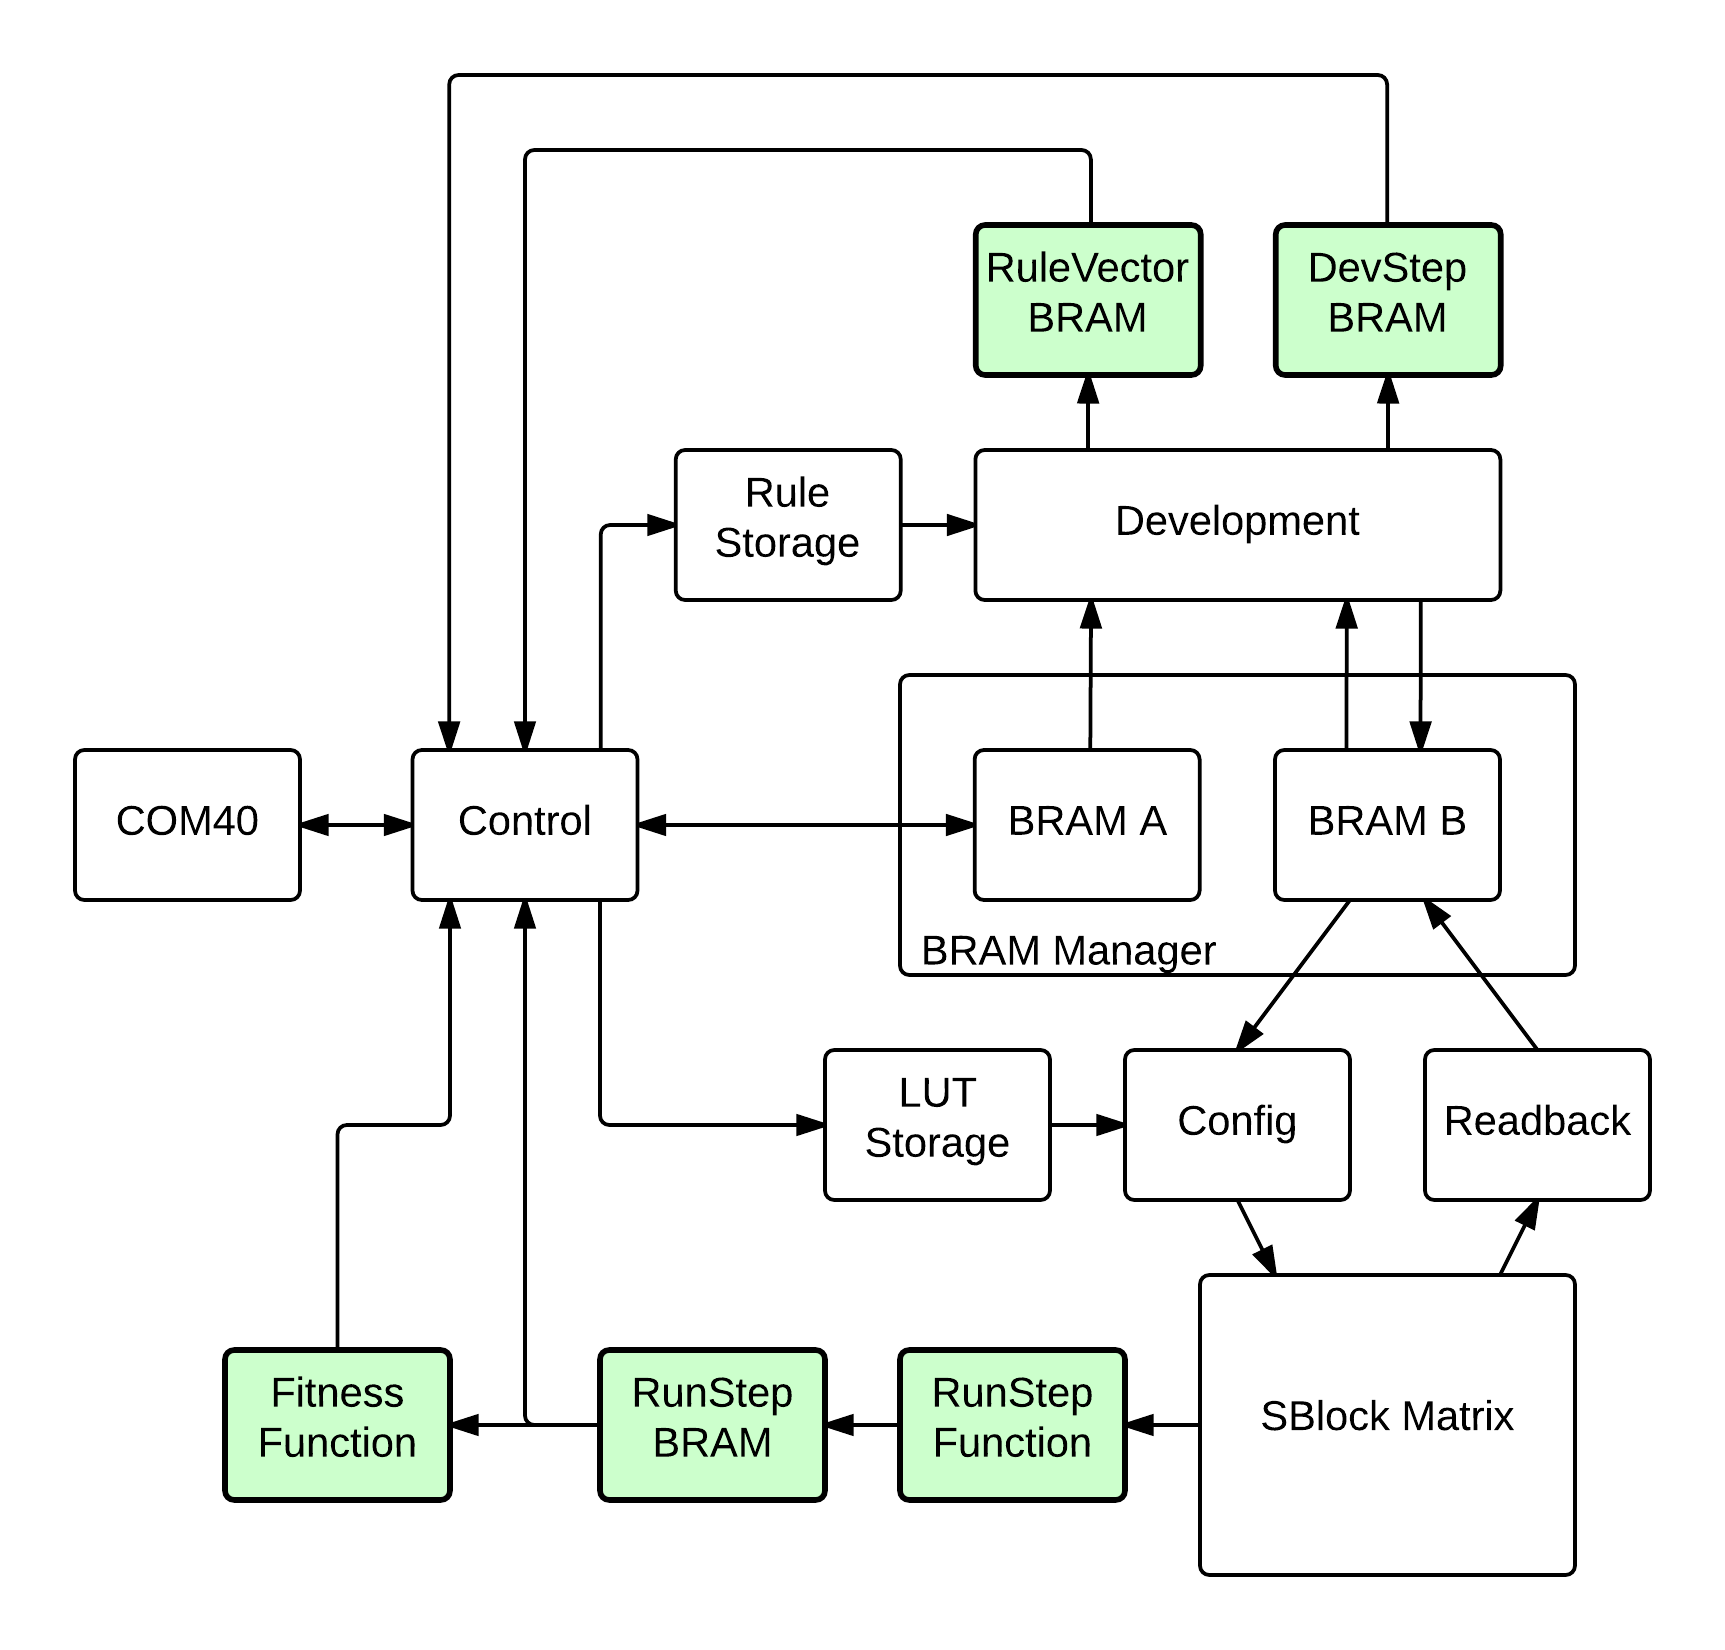
\includegraphics[width=0.48\textwidth]{figures/overview-aamodt}
    \caption{High-level block diagram of the hardware platform after Aamodt's work. Additions are highlighted in green.}
    \label{fig:overview-aamodt}
\end{figure}

The rule vector BRAM stores lists of which rules were triggered and not for the last 256 development steps.
The lists are implemented as bit-vectors where each bit represents the status of a rule for a single development step.
The development step BRAM is more detailed; it stores which rule was triggered for each cell.
However, it only has storage space for one development step.

The run-step function calculates the number of live cells after each SBM update by using a large adder tree.
The numbers are stored in run-step BRAM for later usage by the fitness function, which is replacable.

\subsection{Renovation}

In expectation of receiving new hardware with a larger and faster FPGA, there was a demand to optimize the platform by taking advantage of the increased resource pool.
Extending the platform into the third dimension was also a lucrative thought, as doing so allows more complex signal pathways to form within the cellular automata.
It was also desired to have a discrete fourier transform (DFT) for interpretation of the RSF data; it should give very useful data according to Berg's research \cite{berg2013ca}.
The task of realizing this was taken on by Støvneng \cite{stovneng2014sblock}.

An overview of the hardware platform with Støvnengs additions and optimizations is shown in \figurename~\ref{fig:overview-stovneng}.
The only addition is the DFT, but nearly all units has been optimized, yielding a speedup of 4 for most operations.

\begin{figure}[!ht]
    \centering
    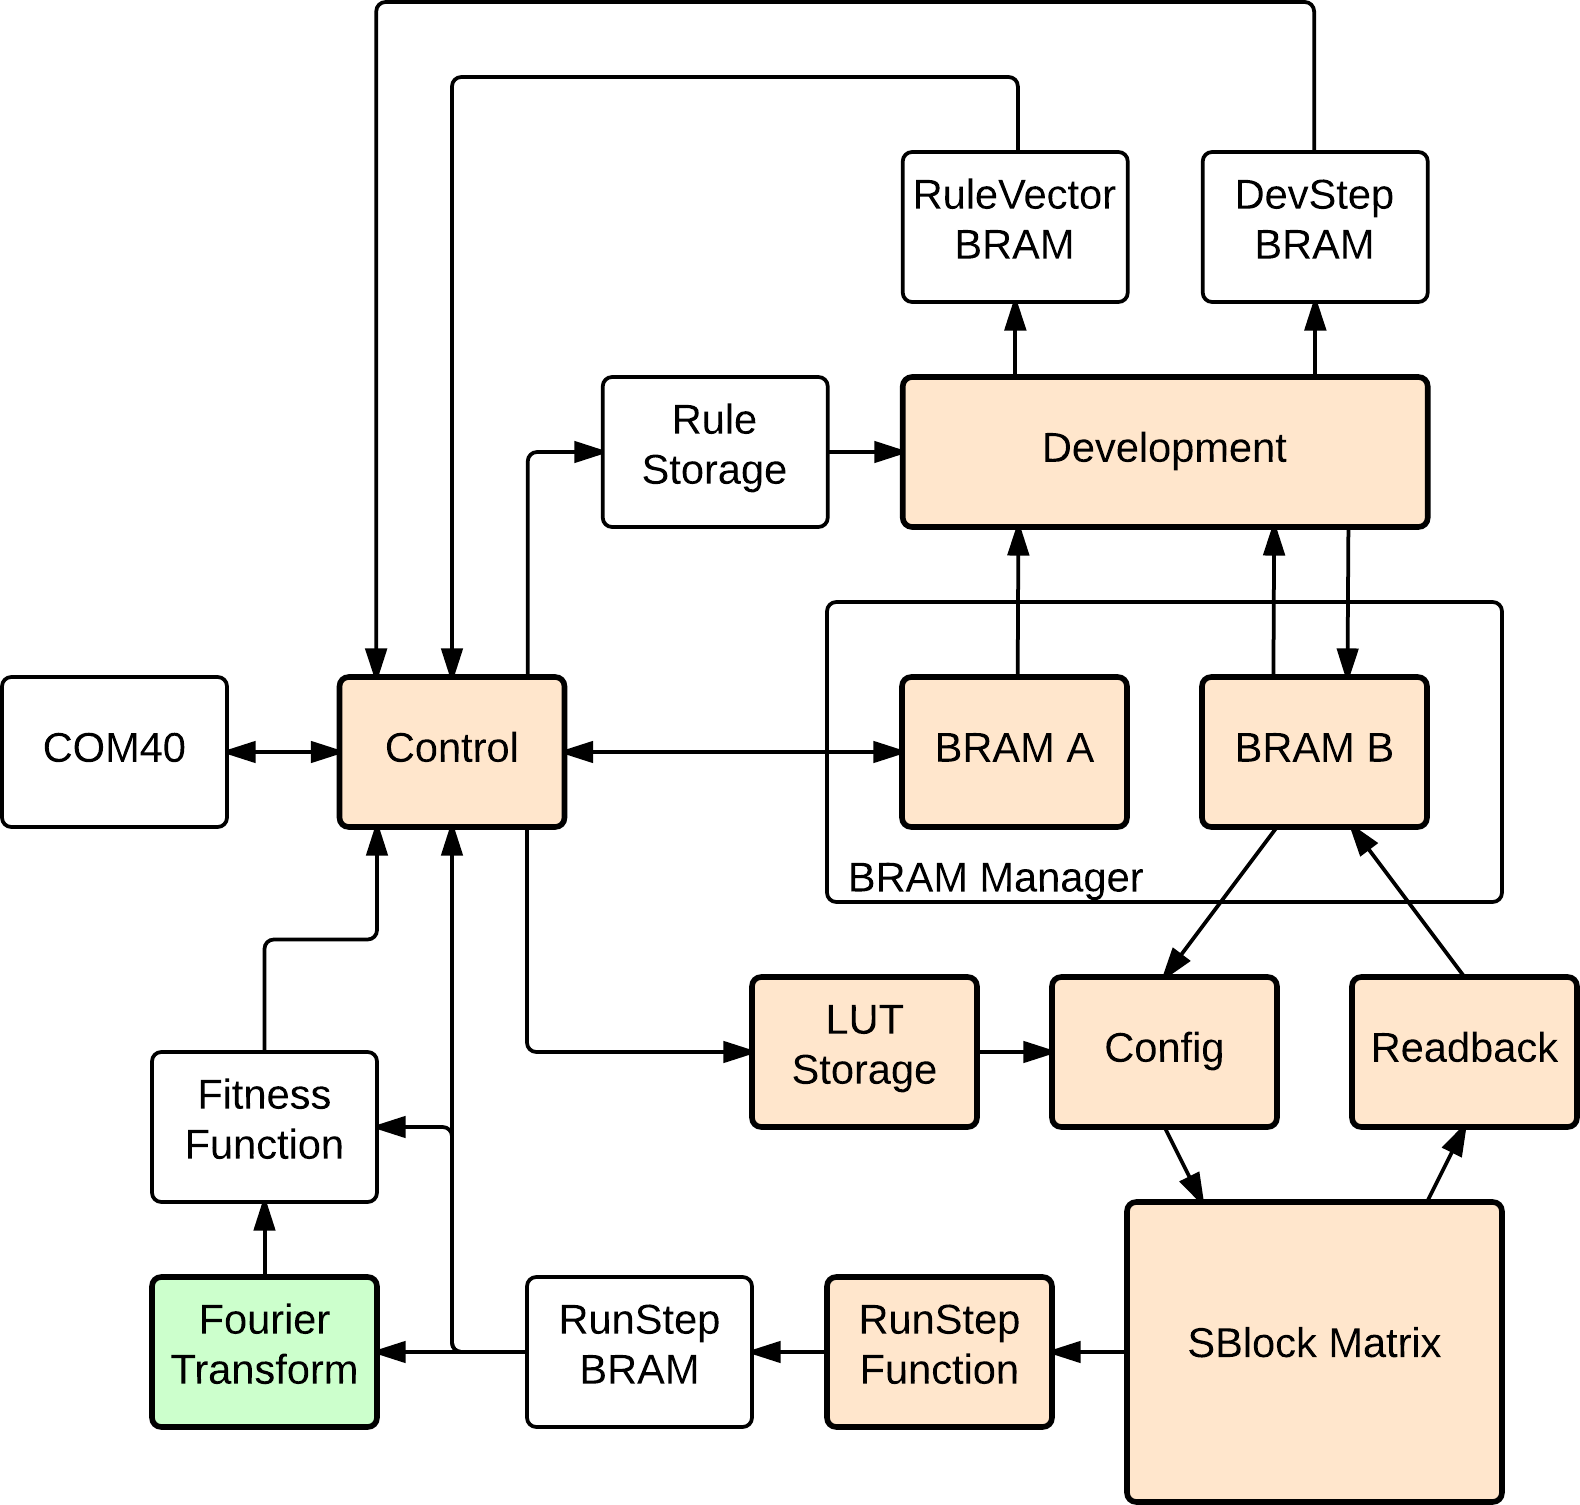
\includegraphics[width=0.48\textwidth]{figures/overview-stovneng}
    \caption{High-level block diagram of the hardware platform after Støvneng's work. Additions are highlighted in green, and optimizations and 3D modifications in orange.}
    \label{fig:overview-stovneng}
\end{figure}

Unfortunately, due to some challenges with manufacturing, Støvneng was unable to get hold of the new hardware for the duration of his project.
The system was therefore only verified in simulation, and the PCI communication unit was not upgraded for the PCI Express connection on the new board.



\section{Motivation}

    \todo{motivations for having a CA research platform}

\todo{rewrite this}

Currently, CARP is only usable in simulations.
They are extremely slow, so it is practically unusable.

Implementing communication should make the new platform operational, allowing it to be used for research.
The new platform is about 4 times faster than the old and support larger sblock matrices.
It also has the new and exciting DFA, which is shown to produce very useful data.
3D is also exiting as it allows much more complex communication pathways inside the CA.

Verification of previous modifications are necessary since it was only tested in simulation.
What works in simulation does not necessarily work in implementation.



\section{Development Platform}

    Multiple weeks into this project, several months after the end of Støvnengs project, there were still no signs of the new hardware.
To prevent the project from halting dead in its tracks, a decision was taken to order slightly different hardware.
The significant difference to the original system is reduced size of the FPGA, a Spartan-6 LX45T instead of a Spartan-6 LX150T, which entails around 70\% less available resources.
Luckily, the hardware design can be scaled down to fit the smaller chip by reducing the size of the sblock matrix, allowing for implementation of PCI Express and verification of the complete system in hardware.

\subsection{Spartan-6 SP605 Evaluation Platform}

The Spartan-6 SP605 Evaluation Platform is essentially a board with the Spartan-6 LX45T FPGA wired to every useful peripheral imaginable.
It has connections for PCI Express\footnote{
        Even though the PCI Express finger has lines for power, they are not connected on the SP605. This means an external power source has to be connected.
    }, ethernet, DVI, USB, flash card, JTAG, LEDs, switches, and more.
However, the only peripherals utilized in this paper are PCI Express, and JTAG.
An overview of the system is shown in \figurename~\ref{fig:sp605}.

\begin{figure}[!ht]
    \centering
    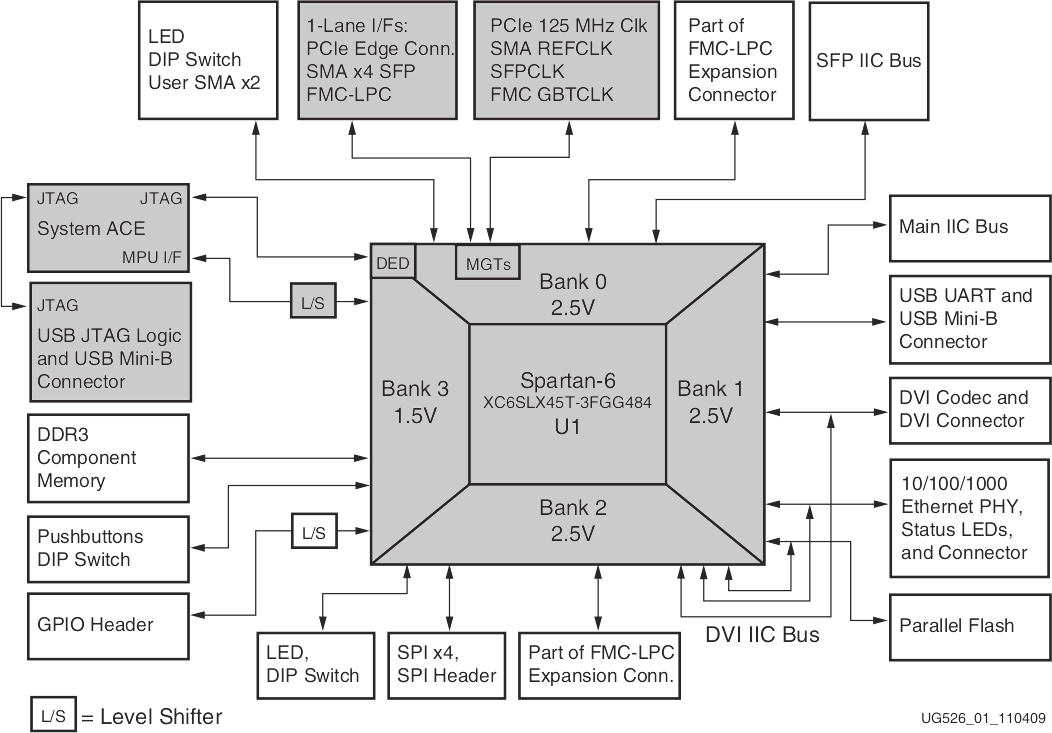
\includegraphics[width=0.48\textwidth]{figures/sp605-modified}
    \caption{High-level block diagram of the SP605 and its peripherals. Peripherals utilized in this paper are highlighted in gray. (Modified reprint from \cite{ug526})}
    \label{fig:sp605}
\end{figure}

The switch and jumper configurations of the SP605 are set to factory defaults, with the exception of SW1 which is set to 10.

\subsection{Hardware setup}

Due to the experimental nature of testing a new hardware platform, two computers were used in this project, as shown in \figurename~\ref{fig:hardware-setup}.
One is the main development workstation, used for coding and synthesis; it has a JTAG connection to the SP605 over USB, which allows it to upload new designs.
The other is the host for the SP605, which is mounted in a PCI Express expansion slot.

\begin{figure}[!ht]
    \centering
    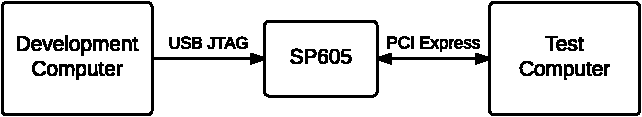
\includegraphics[width=0.40\textwidth]{figures/hardware-setup}
    \caption{High-level block diagram of the hardware setup.}
    \label{fig:hardware-setup}
\end{figure}

The setup allows a new design to be uploaded and tested on the SP605 without disrupting the workflow of the main workstation, due to the power-cycle required to reset the PCI Express connection.

\subsection{Software setup}

The operating system on both computers is Linux Mint; version 16 on the development computer and 17 on the test computer.
Linux Mint is currently one of the most popular linux distributions, along with Ubuntu, which it is based upon \cite{distrowatch}.
This means that procedures and software used and created in this paper should work on most systems.

Xilinx ISE version 13.3 was used for hardware design and synthesis, while ISim was used for simulations.
The third-party USB cable driver from \cite{usbdriver} was used for JTAG, as explained in Section~\ref{sec:challenges}.
The software API was compiled with GCC version 4.8.2.



\section{Communication}

    
Due to the difference in wordsize between the old and new communication unit, a compatibility layer is added to allow other existing code to remain unchanged.

\figurename~\ref{fig:overview-lundal} shows the changes to the hardware platform.
The old COM40 unit has been replaced by a new communication unit and a compatibility layer.
The compatibility layer is needed because the old COM40 unit was based on 64-bit data while PCI Express uses 32-bit data.
\todo{rewrite this}

\begin{figure}[!ht]
    \centering
    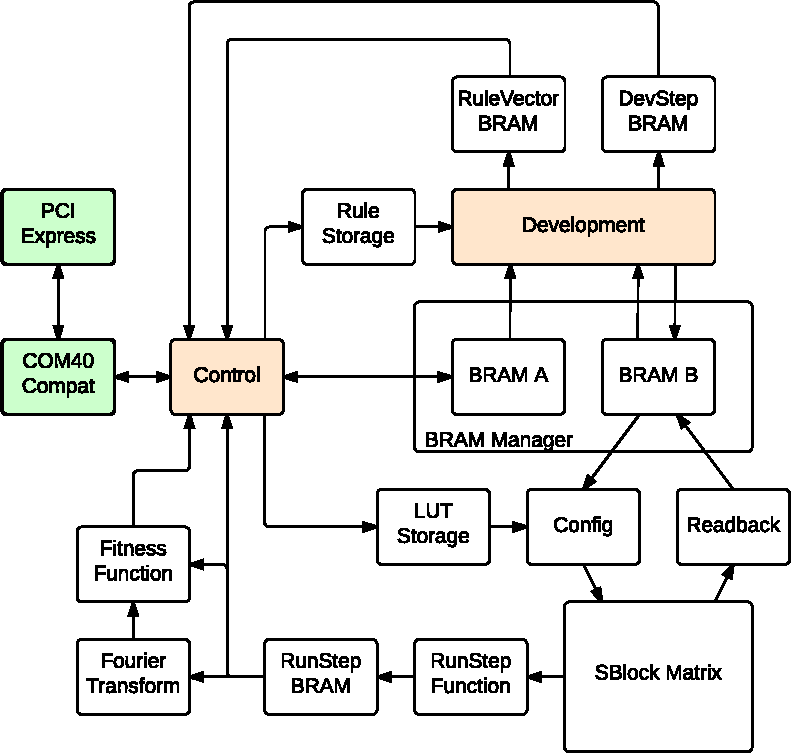
\includegraphics[width=0.48\textwidth]{figures/overview-lundal}
    \caption{High-level block diagram of the current hardware platform. Additions are highlighted in green.}
    \label{fig:overview-lundal}
\end{figure}

The communication unit has internal data buffers.

On the software side, the api uses linux' built-in drivers for PCI Express.

\subsection{Overview}

The new communication unit is based on Xilinx' reference PCI Express programmed io design.
It consists of the Xilinx PCI Express endpoint core, reception and transmission engines, data buffers, and a special request handler, as shown in \figurename~\ref{fig:details-communication}.

\begin{figure}[!ht]
    \centering
    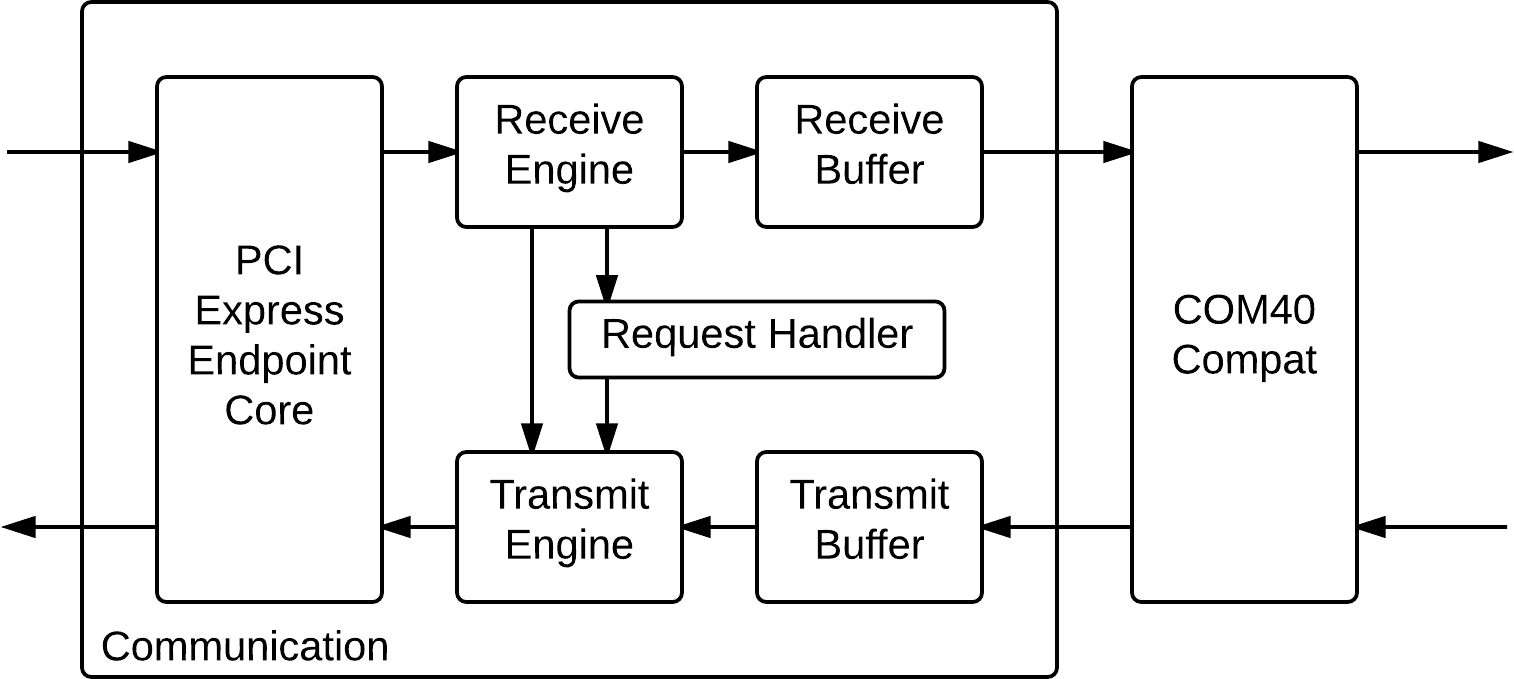
\includegraphics[width=0.48\textwidth]{figures/details-communication}
    \caption{Detailed block-diagram of the PCI Express communication module.}
    \label{fig:details-communication}
\end{figure}

The endpoint core completely handles the physical and data link layers, and all TLPs related to configuration and establishment of the PCI Express connection.
Other TLPs, such as read and write requests, are presented on an AXI4-Stream interface \cite{ug672}.
The reception engine is responsible for parsing TLPs and either writing received data to the reception buffer or notifying the transmission engine about a read request.
The transmission engine is responsible for building completer TLPs to respond to read requests, using data from the transmission buffer.
The request handler listens to the read requests provided by the reception engine, and can override the transmission engine to respond to special requests.

\subsection{PCI Express Endpoint Core}

Several Spartan-6 FPGAs, including the one used in this project, contain a special-purpose hardware block for implementation of PCI Express.
The block completely handles the physical and data link layers, with the transaction layer left for the user.

To make use of the block, Xilinx provides the Spartan-6 Integrated PCI Express Endpoint Core; version 2.3 was used in this project.
This core additionally takes care of all TLPs related to configuration of the PCI Express connection.
Other TLPs, such as read and write requests, are presented on an AXI4-Stream interface \cite{ug672}.

The endpoint core is configured with two memory regions, both 4 kB in size\footnotemark.
\footnotetext{
    The smallest memory region that can be memory-mapped is one page. The default page size in Linux is 4 kB.
}
The first memory region (BAR0) is used for normal communication, while the second (BAR1) is used for special requests.
The separaton is mostly conseptual as both regions are treated like a singular stream.
The difference is that the special request handler kicks in for read requests to BAR1.

\todo{wrapper?}
\todo{vendor/device id?}

\subsection{Reception engine}

The reception engine is implemented as a simple state machine, as shown in \figurename~\ref{fig:statemachine-receive}.

\begin{figure}[!ht]
    \centering
    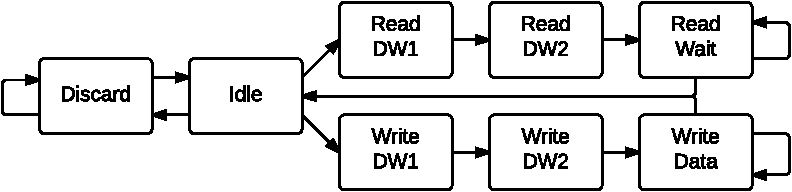
\includegraphics[width=0.48\textwidth]{figures/statemachine-receive}
    \caption{State machine for the reception engine.}
    \label{fig:statemachine-receive}
\end{figure}

Until the endpoint core presents valid data, the state machine remains in Idle.
When it does, the data is stored, and the TLP type is checked.
If it is a read or write request, the state machine continues down the corresponding path, otherwise the remaining data is discarded.
The remaining portion of the TLP headers are then parsed in the DW1 and DW2 states.
For read requests, the state machine waits in ReadWait until the transmission engine is ready to accept a new read request, and then proceeds to Idle.
For write requests, the state machine stays in WriteData, where one DW of data is written to the reception buffer each cycle, for the length of the packet, and then proceeds to Idle.

\subsection{Transmission engine}

The transmission engine is implemented as a simple state machine, as shown in \figurename~\ref{fig:statemachine-transmit}.

\begin{figure}[!ht]
    \centering
    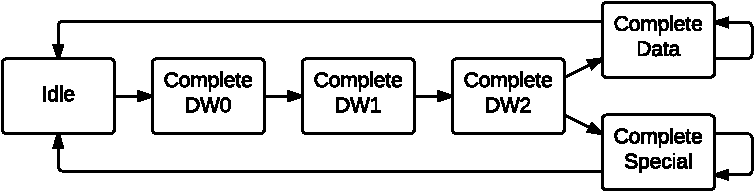
\includegraphics[width=0.48\textwidth]{figures/statemachine-transmit}
    \caption{State machine for the transmission engine.}
    \label{fig:statemachine-transmit}
\end{figure}

Until the reception engine signals a read request, the state machine remains in Idle.
When a read request is signaled by the reception engine, the state machine begins to traverse the DW path.
The DW0, DW1 and DW2 states each transmit one DW of the completer TLP header.
Then if the special request signal is set, it procceds to CompleteSpecial, where it transmits data presented by the request handler.
Otherwise, it proceeds to CompleteData where it transmits one DW of data from the transmission buffer each cycle.
When the requested number of DWs has been transmitted it proceeds back to Idle.

\subsection{Request handler}

The request handler continually listens to the read requests presented by the reception engine.
If the request is targeting the primary memory area (BAR 0), it is a normal read request and the transmission engine is allowed to proceed as usual.
Otherwise, it is a special request and the transmission engine is overridden.

The kind of special request is determined by the address of the read request, and handled thereafter.
There are currently four special requests implemented, as shown in Table~\ref{tab:requests}.

\begin{table}[!ht]
    \renewcommand{\arraystretch}{1.3}
    \caption{Special requests}
    \label{tab:requests}
    \centering
    \begin{tabular}{c|l}
        \bfseries Address & \bfseries Request \\
        \hline
        0x00 & Get transmission buffer data count \\
        0x01 & Get transmission buffer available space \\
        0x02 & Get reception buffer data count \\
        0x03 & Get reception buffer available space \\
    \end{tabular}
\end{table}

Note that each of the implemented special requests assumes a read request length of one DW.
If the request has a greater length, the returned data is simply repeated that number of times.

\subsection{Buffers}

The buffers are implemented as first-in first-out (FIFO) queues using block RAM (BRAM) and two counters.
The counters deterimine the addresses that are written to and read from, and are incremented when the write or read signals are asserted.
\figurename~\ref{fig:wavediagram-fifo} shows how the FIFO is used to buffer two words.

\begin{figure}[!ht]
    \centering
    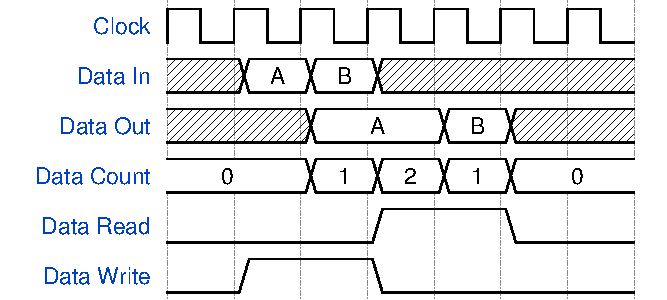
\includegraphics[width=0.40\textwidth]{figures/wavediagram-fifo}
    \caption{Wave diagram for the FIFO buffer, showing two consecutive writes followed by two consecutive reads.}
    \label{fig:wavediagram-fifo}
\end{figure}

Notice how the read signal needs to be asserted before the clock tick when data is read to ensure correct consecutive reads.
This is due to the BRAM used in the FIFO, which updates at clock ticks.
To have correct data available for a read in the following cycle, the address therefore has to be updated before the clock tick (by asserting the read signal).

\subsection{Software API}

The communication part of the new software API is split into two parts.

The first is a general interface for connecting to PCI and PCI Express devices without using a custom driver.
It takes advantage of Linux' automatic population of /sys/devices/pci* with files representing the memory regions of all PCI and PCI Express devices.
The directory is searched by vendor and device id, and the corresponding memory regions is memory-mapped into the program.

The second is an interface specifically for the communication unit.
It provides open, close, read and write functions similar to the old BenERA interface, in addition to implementing all special request functions in Table~\ref{tab:requests}.
When a read or write operation is initiated, buffers are checked for available data or space.
If there is not enough present, the program waits and then rechecks.



\section{Verification}

    Due to lack of hardware, Støvneng only verified his changes in simulation.
With available hardware and an updated communication unit, the design can finally be properly verified.

\subsection{Methodology}

The communication unit was tested in hardware by connecting the output of the reception buffer to the input of the transmission buffer.
Then sample data was sent over PCI Express to the SP605 and then read back.

The updated hardware design was tested with SBM sizes of 8x8 for 2D and 8x8x8 for 3D.
The tests are detailed in Appendix \ref{sec:tests}; each one has a short description and a list of the instructions it verifies.
Together, the 11 tests cover all instructions.

Note that due to some instructions being dependent on others, it is not always possible to know which instruction is failing.

\subsection{Results}

The communication unit returns the correct data in the correct order, which means it passes its test.

The 2D design passes all tests except for 6 and 8, while the 3D design failes test 1, 3, 6, 7 and 8.
This means that the two most crucial components, the SBM and development unit, is working in neither.
The 3D design also has some additional issues.

The status of each instruction is listed in Table~\ref{tab:instructions}, while descriptions of the issues are listed in Section~\ref{sec:remaining-issues}.

Some issues were solved in the alotted time.
They are not included in these results, but are listed in Section~\ref{sec:solved-issues} for completeness.

\begin{table}[!ht]
    \renewcommand{\arraystretch}{1.3}
    \caption{Implementational status of instructions}
    \label{tab:instructions}
    \centering
    \begin{tabular}{l|l|l}
        \bfseries Instruction & \bfseries Works in 2D & \bfseries Works in 3D \\
        \hline
        break & Yes & Yes \\
        clearBRAM & Yes & Yes \\
        config & Yes & Undecidable \\
        devstep & Undecidable & Undecidable \\
        doFitness & Undecidable & Undecidable \\
        end & Yes & Yes \\
        jump & Yes & Yes \\
        jumpEqual & Yes & Yes \\
        nop & Yes & Yes \\
        readback & Yes & Undecidable \\
        readFitness & Undecidable & Undecidable \\
        readRuleVector & No & No \\
        readState & Yes & Yes \\
        readStates & Yes & Yes \\
        readSums & Undecidable & Undecidable \\
        readType & Yes & Yes \\
        readTypes & Yes & Yes \\
        readUsedRules & Undecidable & No \\
        resetDevCounter & Yes & Yes \\
        run & Undecidable & Undecidable \\
        setNumberOfLastRule & Undecidable & Undecidable \\
        startDFT & Undecidable & Undecidable \\
        store & Yes & Yes \\
        switch & Yes & Yes \\
        writeLUTConv & Undecidable & Undecidable \\
        writeRule & Undecidable & Undecidable \\
        writeState & Yes & Yes \\
        writeStates & Yes & No \\
        writeType & Yes & Yes \\
        writeTypes & Yes & No \\
    \end{tabular}
\end{table}

\subsection{Remaining issues}
\label{sec:remaining-issues}

\emph{ReadStates prints garbage in top 32 bits.}
This occurs due to a buffering error in the LSS unit.
However, only the least 32 bits are used by the api, which means that this issue only impacts performance and not functionality.

\emph{WriteStates and WriteTypes does nothing in 3D.}
This issue is only present on the board, not in any simulations, which makes it hard to track down the cause.

\emph{ReadRuleVector sends incorrect data.}
The first execution of the instruction produces an extra word; a repetition of the first.
Following executions produces the correct amount of words, but the order is offset by one.

\emph{ReadUsedRules fails for SBM widths less than 16.}
The simulator crashes with an index-out-of-bounds error, due to the instruction treating a $[width\cdot4]$ bits wide signal as if it is 64 bits wide.
How ISE is able to implement the design despite illegal indexing is a mystery, but the instruction produces only zeroes when executed on the board.

\emph{Development rules does not activate.}
This issue is also only present on the board, making it hard to analyze.
The root cause could be with any of the following instructions: devstep, writeRule and setNumberOfLastRule.

\emph{Config does not properly write states in 3D.}
Simulations show that the BRAM address fluctuates, causing the states to be overwritten by 0 in the following cycle.

\emph{Runstep causes every state to become zero.}
When a runstep is performed, all states in the SBM is reset to 0.
\todo{present in sim?}

\subsection{Solved issues}
\label{sec:solved-issues}

\emph{States and types were written to the wrong location.}
When writing single states or types, a half-row is read from BRAM, combined with the new data, and written back to BRAM.
Due to the usage of non-implementable code to specify how the data should be combined, the new data always ended up in the middle of the half-row.

\emph{Development ran indefinitely.}
Comparison of signals of different widths always return false.
Due to the comparison of a parameterized signal with a constant, the development unit would not iterate through the cells, and thus never finish.

\emph{WriteRule did not follow spesification.}
When the api transformed a 3D rule struct into an instruction, the position of up/down and north/south were swapped.

\emph{PrintTypes used wrong offsets for decomposition.}
When decomposing a row of types into individual types, an offset of 5 was used instead of 8.
This entailed that the printed values appeared as garbage.

\emph{ReadVector and PrintVector used 32-bit words.}
The functions were not updated from using 32-bit to 64-bit words.
ReadVector would therefore expect twice the number of words provided by the hardware platform, causing the program to wait for nonexistant data.



\section{Discussion}

    \todo{add section intro}

\subsection{Challenges}
\label{sec:challenges}

There was a lot of concern during initial hardware testing, as the SP605 was not detected by the computer.
A slightly curved circuit board led to the beilief that there might be something wrong with hardware.
Luckily, it proved not to be a hardware fault, but a mistake in the hardware setup guide; the position of SW1 was reversed, causing the board to operate in a completely different mode.

The SP605 was pre-installed with an example design implementing communication over PCI Express with DMA.
However, the accompanying driver did not support newer linux kernels.
Additionaly, the design was written in verilog while CARP is written in vhdl, which meant extra effort to integrate the two.
There was some effort applied to update the driver, but it was abandoned due to near-untraceable segfaults.

The USB cable driver for usage of JTAG provided by Xilinx also had the problem of not being compatible with newer linux kernels.
Thankfully, a the driver found at \cite{usbdriver} is compatible and solves the problem.

\todo{Development bug}

\begin{itemize}
    \item Works in post-translate sim
    \item Doesn't work on dev board
    \item All post-map and post-par simulations give X'es
    \item Can't keep\_hierarchy to trace source
\end{itemize}

\subsection{Future work}

The most important thing going forward is to fix the errors that are preventing the sblockmatrix and development units from working correctly.
However, this is no easy task, as large parts of the design are highly complex and difficult to debug.
The most extreme cases are the development and LSS units which each consists of a single large file, around 1200 lines long, of complex pipelined code.
Simplification and modularization of these units is therefore imperative.

Another reason to simplify the development unit is it's extreme memory bandwidth requirement against the SBM BRAM.
Currently, the it is designed so that N rules are loaded, applied to every cell, then the N next rules loaded and so on.
This means that the SBM BRAM must supply 5 rows each cycle to test 1 row per cycle (or 8 for 2) in 3D, while N rules are needed per matrix iteration.
In addition, after the first pass, cells has to be read from BRAM B instead of BRAM A, since some cells might have changed.

A simplified process would be to read 5 rows, apply one rule to the center row each cycle, then read the next 5 rows, and so on.
This will greatly lessen the bandwidth requirements against the SBM BRAM, as the rows can be read in sequence while each rule is being applied.
Assuming there are more rules than the number of rows that must be read (highly likely), there is no performance loss.
Additionally, this would allow development to only read from BRAM A.

There are still some remains of having two clock domains, more specificaly a pair of flipflops used for clock-synchronization in the fetch and lss units.
It does not affect functionality, and has therefore been of low priority, but it does add a slight delay between the communication unit and the fetch and lss units when reading data.

Currently, the platform only supports dimension sizes that are powers of 2.
It would be beneficial to be able to select any size, allowing for fine-tuning of the resource usage, to get most out of the FPGA.

As noted in \cite{stovneng2014sblock}, Støvneng increased the base instruction and data sizes from 32 to 64 bits.
Although it is one way to accomodate for longer instructions, the decision is a little odd, considering both PCI and PCI Express are based on 32-bit word sizes.
This means that conversion is currently required between the LSS and communication units.
Since only 6 out of 30 instructions require more than 32 bits, communication could be simplified and optimized by going back to a 32-bit base size.

Finally, a unification of the 2D and 3D designs would be \TODO

\begin{itemize}
    \item Com buffer checks
    \item Get rid of tristate buffers \cite{koch2008buses}
    \item Get rid of reset (init values in \cite{ug687} page 55-56, \cite{wp272} page 5)
    \item Use generics instead of global constants
    \item Unify 2D and 3D designs
    \item Add instruction that reports info (2D/3D, SIZE, ++)
    \item Add general purpose counters
    \item DMA (better performance?)
    \item Toggle SBM wrap-around
\end{itemize}

With the current need for major fixes, simplification of development and LSS, reducing the need for extreme memory bandwidth, removing tristates, removing resets, and unification, it might be a good idea to rebuild the platform from the ground up.
Starting from a clean slate, thoroughly evaluating every part of the design, replacing the bad features and improving the good, will likely result in a greatly improved platform for CA research.



\section{Conclusion}

    \todo{rewrite this}

PCI Express communication has been implemented - both in hardware and software.
It is tested, and works beautifully.

Verification shows that Støvnengs work has resulted in a lot of implementational issues.
Some were able to be fixed in this project, others not.



\bibliographystyle{IEEEtran}
\bibliography{IEEEabrv,bibliography}

\todo{appendices: tests, files, ?}

\end{document}

